\section{Analysis - Total Interaction Cross Section $^{12}$C + $^{12}$C - $^{12}$C + $^{12}$C}
This chapter will go through the  analysis step by step from the unpacking stage to the final measurement of the total reaction cross section. It will start by a short overview of the transmission method used for the cross section measurements. The next step is  the selection of clean incoming $^{12}$C isotopes. Following the identification of the carbon isotopes after the target - for the measurement of the charge changing cross section - and as final step the reaction cross section measurement. \newline
All relevant detector related geometrical and efficiency corrections will be adressed and their influence to the final result and its uncertainty will be discussed.
\subsection{Cross Section Measurement via Transmission Method}
In its most generic form cross sections give a measure of the probability that a specific reaction will take place when two or more particles collide. The cross sections  measured in scattering exepriments, as well as the energy and angular distribution of the reaction products, provide information about the dynamics of the interaction between the projectile and the target particle, i.e., about the shape of the interaction potential and the coupling strength.\newline
The cross section $\sigma$ can be derived by looking at the relation between the number of incoming particles (N$_{1}$) and unreacted particles after collision ($N_{2}$). For an experiment with fixed target with thickness $z$ and volumetric number density $n$ the number of reacted particles in the infinitesimal thin target layer $dz$ can be expressed as:
\begin{equation}
\frac{dN_{2}}{dz} = -n \sigma N_{2}
\end{equation}
Solving this differential equation for $N_{2}$ (with the condition $N_{2}$ = $N_{1}$ for $z=0$) discloses an exponential relation:
\begin{equation}
N_{2} = N_{1}e^{-n\sigma z}
\label{eq:cross_sec}
\end{equation} 
Where $n z$ can be summarized as $N_t$, the total number of scattering centers per unit area. The relation $(N_{2}/N_{1})$, number of unreacted particles after collision versus number of incoming particles, is often called survival probability. For an idealistic experimental setup with full detector efficiency and no interactions in the setup material the cross section could simply be deduced from equation \ref{eq:cross_sec}. To account for reactions of the projectile that occur within the setup material and first order detector specific distortions of output signals the survival probabiltiy $(N_{2}/N_{1})$ has to be divided by $(N_{2}^E/N_{1}^E)$, where $N_{1}^E$ is the number of incoming particles and $N_{2}^E$ the number of unreacted particles after collision for an empty run respectively. The factor $(N_{2}^E/N_{1}^E)$ can also be seen as an overall-experiment specific efficiency. The final formula for the cross section for a so called transmission measurement is:
\begin{equation}
\sigma = -\frac{1}{N_t} ln(\frac{1}{\epsilon_{setup}} \frac{N_2}{N_1}),\quad with \quad  \epsilon_{setup} = \frac{N_{2}^E}{N_{1}^E}
\label{eq:corr_cross}
\end{equation}
From the above formula \ref{eq:corr_cross} it is evident that for cross section measurements with the transmission method three types of observables have to be measured:\newline
\begin{enumerate}
\item[$\blacksquare$] \textbf{Number of scattering centers $N_t$}\newline
The number of scattering centers per unit area of the target is a target specific number. It depends from the target thickness and and its density. The values herefore are taken from \cite{ponnath2023precise}\footnote{For the purpose of this work the target thicknesses were remeasured at GSI with a chromatic sensor giving 2D depth profiles of each target.}. 
\item[$\blacksquare$] \textbf{Number of incoming projectiles ($^{12}$C) $N_1$}
For the measurement only events with well identified incoming $^{12}$C projectiles are chosen. Herefore strict cuts on the detectors upstream the target are set. This strict (upstream) event selection makes sure that we only consider events with single $^{12}$C ...See more in section \ref{subsec:event-sel}.  %TODO finish this sencence 
\item[$\blacksquare$] \textbf{Number of unreacted projectiles ($^{12}$C) $N_2$ after the target}
Detectors downstream the target are used to count the number of unreacted projectiles $^{12}$C. To reduce detector specific influences which could distort the result it is advisable to use only as few as requirable detectors for the clear identification of unreacted projectiles. Moreover detector specific efficiencies which only depend of the beam energy are cancelled out by including both empty and target runs in the cross section calculation, see equation\ref{eq:corr_cross}. For all downstream detectors used in this analyisis it is critical to limit any selection cuts to what is necessary and if necessary systematically check their effects on the counted number $N_2$.
\end{enumerate}
\subsection{Event Selection}\label{subsec:event-sel}
\begin{figure}[htpb]
    \centering
    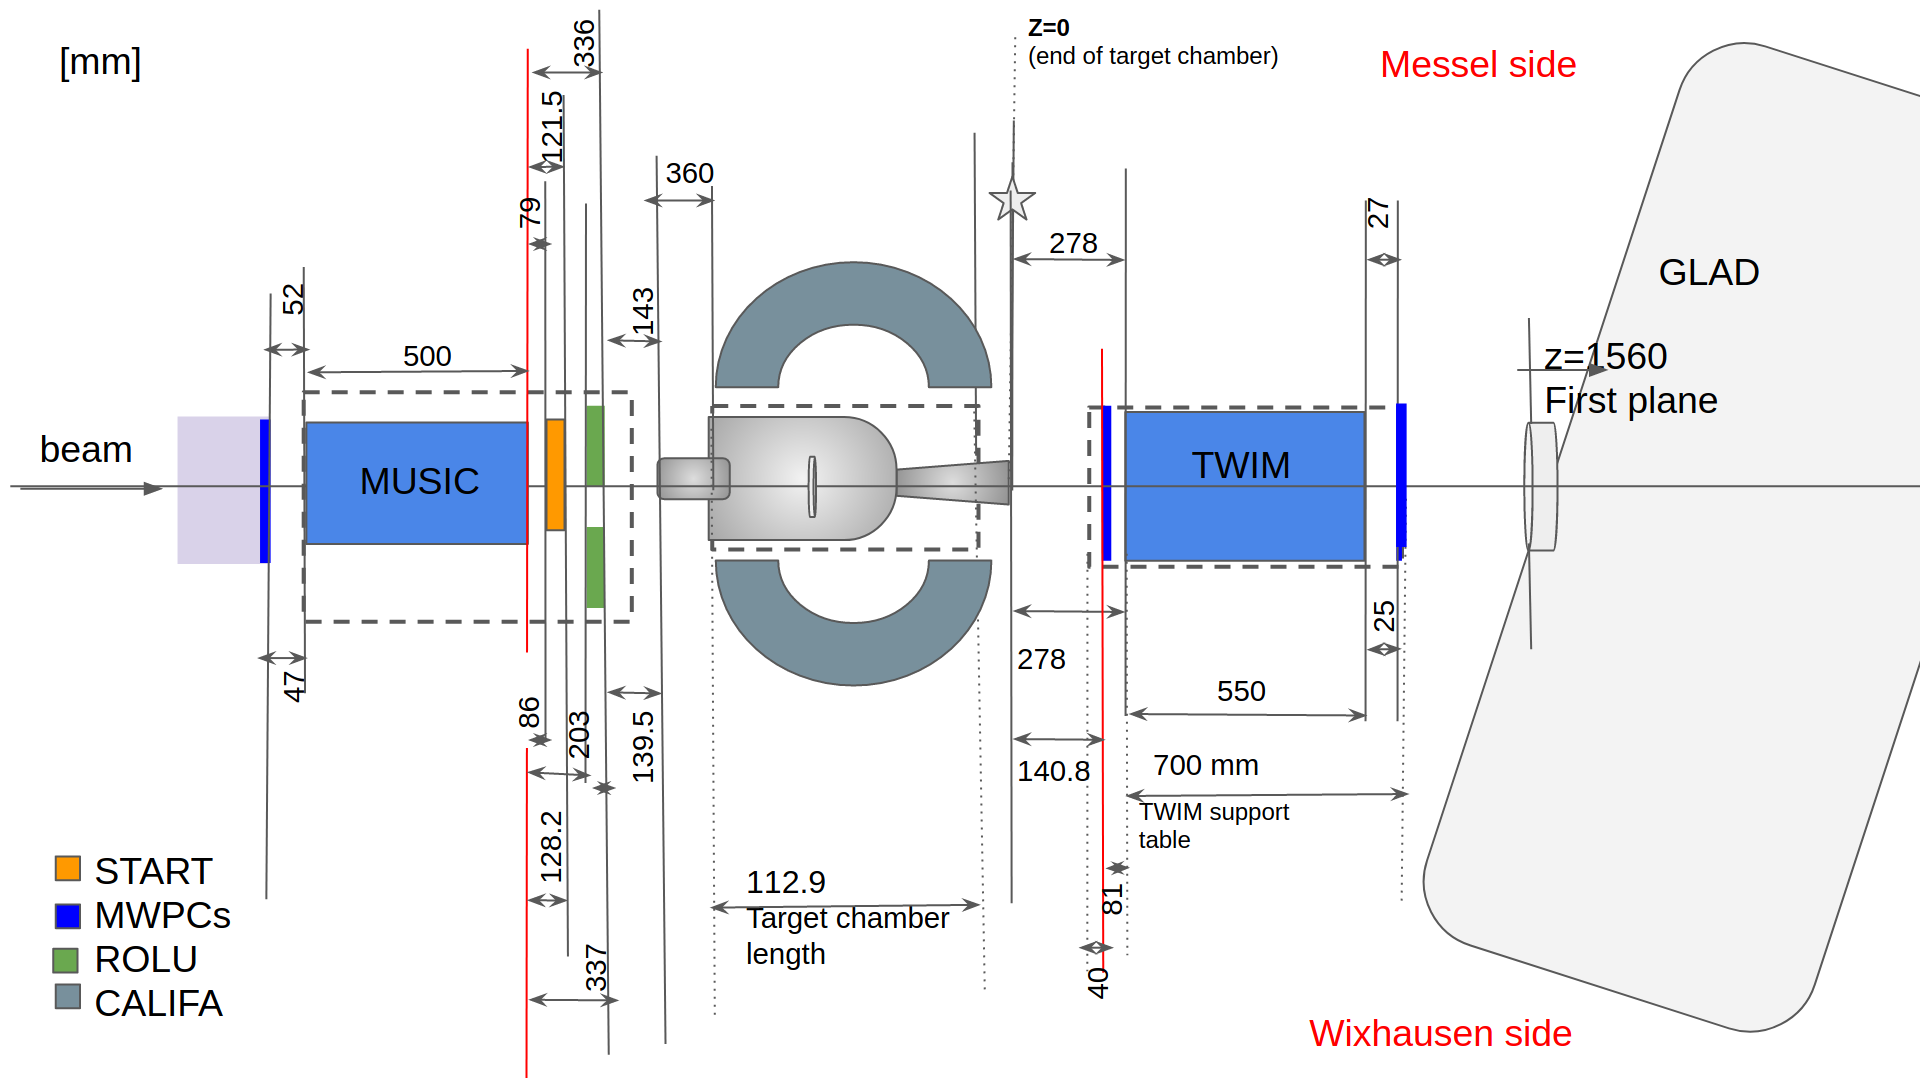
\includegraphics[width=\textwidth,height=6cm,keepaspectratio=true]{Figures/SETUP_around_Target.png}
    \caption{
    R3B Setup for the S444 experiment in the target region. 
    }
    \label{fig:setup_target_region}
\end{figure}

For event selection, all three upstream detectors are utilized: the MWPC0, the R3BMusic Ionization Chamber, and the START detector. To ensure a clean incoming event selection, the following prerequisites must be met:
\begin{enumerate}
\item \textbf{$^{12}$C identification of incoming projectile by upstream detectors:}\newline
\begin{figure}[htpb]
    \centering
    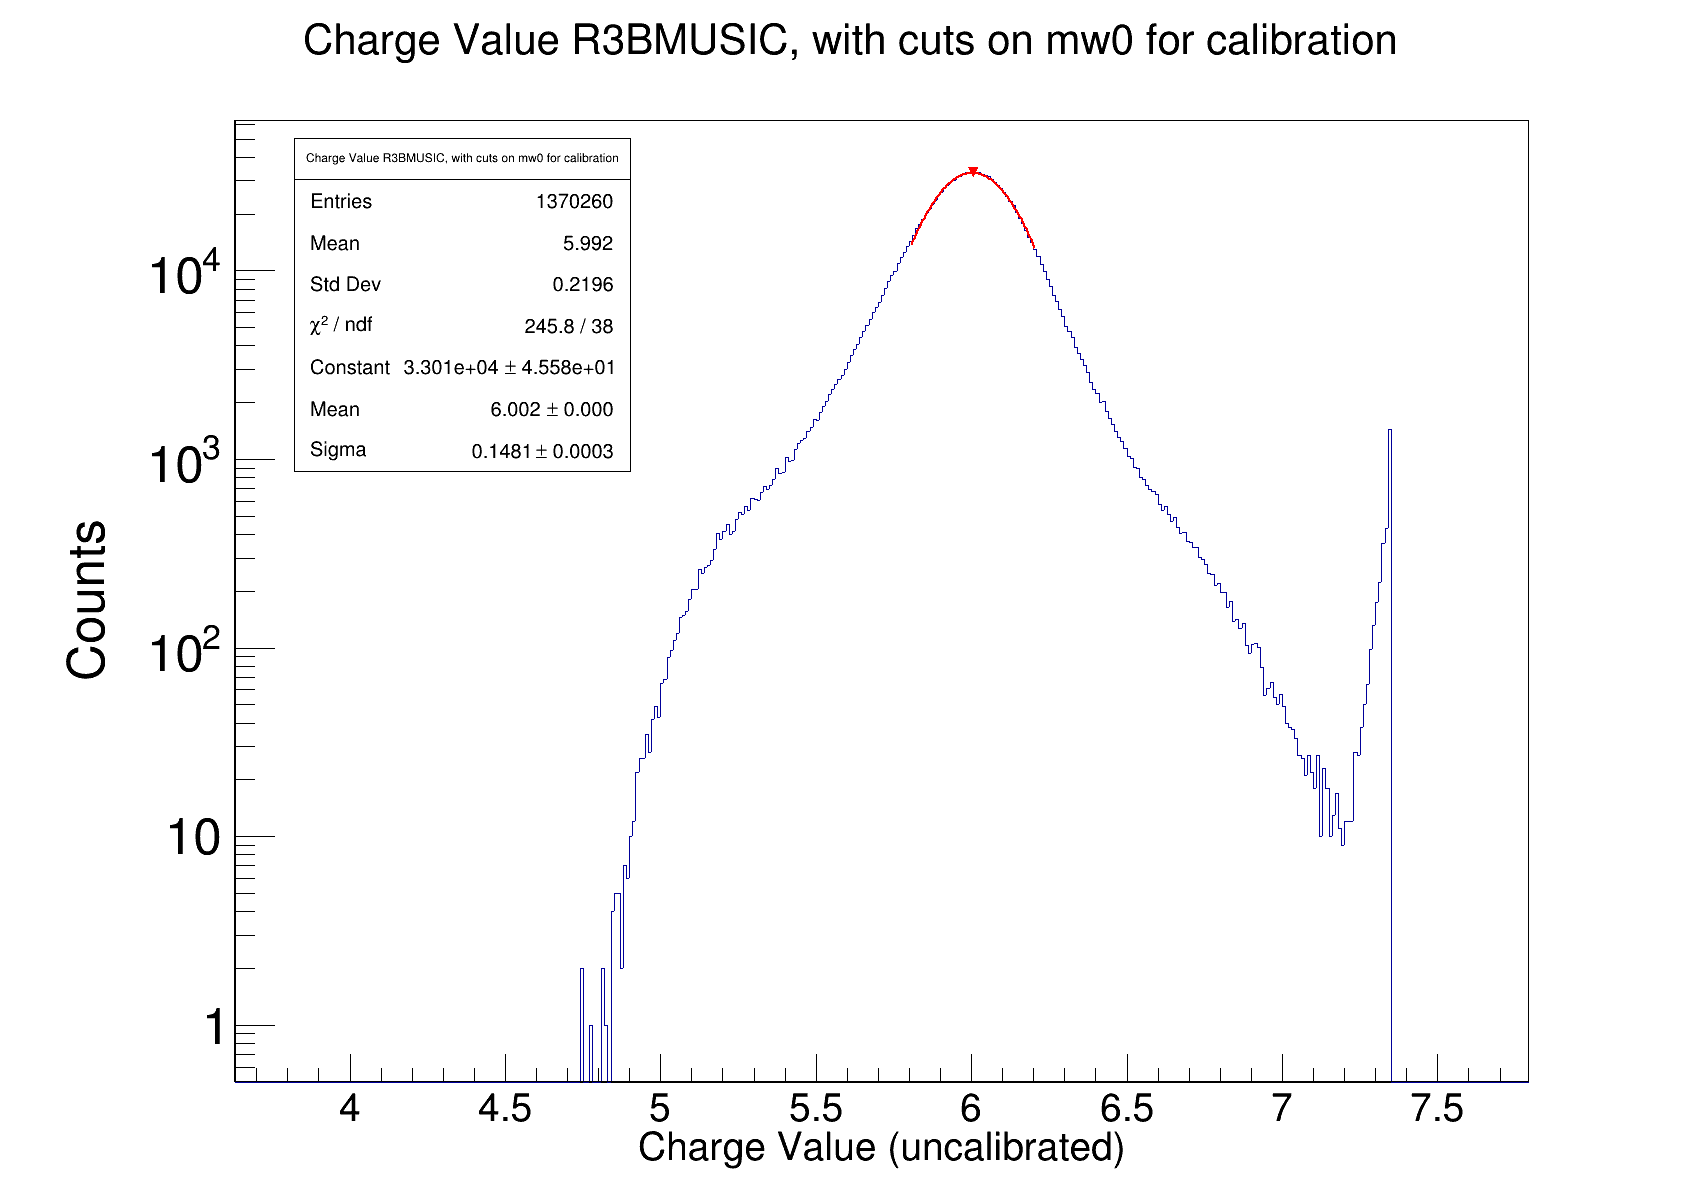
\includegraphics[width=\textwidth,height=8cm,keepaspectratio=true]{Figures/charge_r3bmusic.png}
    \caption{
    Charge distribution on R3BMusic with predefinded calibration parameters with already applied positional cuts on MWPC0 - positioned upstream to the ionisation chamber. 
    }
    \label{fig:r3bmusic_charge}
\end{figure}
In the S444 experiment the incoming beam was directly delivered by the SIS18 ring accelerator, which is operated in ultra-high vacuum the level of pollution is low.(TODO:up to which stage do we have vacuum? Until MW0?)\newline %TODO:up to where is the beam in vacuum?
For the charge identification of the incoming ion the R3BMusic ionisation chamber is used which is positioned directly after the MWPC0 at the beam entrance in Cave C,see figure \ref{fig:setup_target_region}. The R3BMusic detector measures anode-wise the energy loss of the passing-through ion which in the first order is proportional to the square of its charge ($\Delta E \sim Z^{2}$). Herfore the default predefined calibration parameters are used. Figure \ref{fig:r3bmusic_charge} shows the measured charge distribution in R3BMusic. To select $Z = 6$ incoming ions the distibution is fitted. All ions with charge within the $\pm 1 \sigma$ range are accepted. Figure \ref{fig:r3bmusic_cuts} summarizes the $\pm 1 \sigma$ cuts on the R3BMusic charge for empty/target runs for all beam energies.   
\begin{figure}
\centering
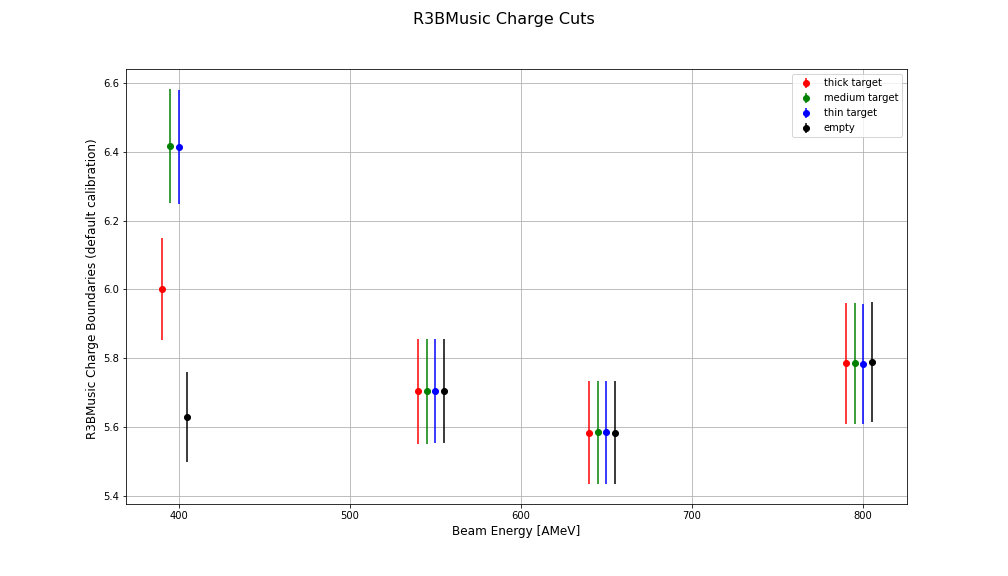
\includegraphics[width=\textwidth,height=8cm,keepaspectratio=true]{Figures/r3bmusic_charge_cuts.png}
\caption{Strict $\pm 1 \sigma$ charge cuts with R3BMusic for incoming particle selection. Fixed predefined calibration parameters were used which do not compensate different gain settings between runs. }
\label{fig:r3bmusic_cuts}
\end{figure}
\item \textbf{Pileup rejection and TPat selection:}\newline
The overall recoding and merging of the data from various subdetectors is one of the tasks of the Data AcQuisition (DAQ) system. Whether an event is recorded or not depends on the pre-established trigger logic. Various detectors can send out triggers to the main DAQ when certain conditions are given (e.g. CALIFA sends aout a trigger when a hit with more than 20 MeV is recorded). The different triggers are processed by the trigger logic and summarized as a defined trigger pattern, so called TPat, which is stored in a 16-bit mask for each event. Table \ref{tab:tpats} gives an overview of the trigger logic and the trigger patterns set in the S444 experiment. For this analysis the \textit{"Min. Bias"} trigger is required\footnote{This includes also \textit{"Reaction"} and \textit{"Neutron"} TPat since these patterns contain also \textit{"Min. Bias"} TPat as necessary condition.}.\newline 
\begin{table}[h!]
\centering
\begin{tabular}{||c c c||} 
\hline
Bit Position &TPat Name & Description \\
\hline\hline
0 & Min Bias & Hit in Start detector\\
1 & Reaction & "CalifaOR" -high energy hit in CALIFA \\
2 & Neutron & Hit in NeuLAND \\
3 & p+n & Hit in CALIFA and Neuland \\
8 & Califa & high energy hit in califa - off-spill \\
9 & NeuLAND & Hit in NeuLAND - off-spill \\
\hline\hline
\end{tabular}
\caption{List of TPats set for S444 experiment. As for the selected runs low beam rates ($< 10kHz$) were expected no dead time issues should arise for the in-beam detectors, therefore no downscaling of the \textit{Min. Bias} TPat was deployed.}
\label{tab:tpats}
\end{table}
Since the TPat selection itself does not necessary set any pileup constraints it is important to analyse the signals of the detectors upstream carefully to insure yourself that only events with  one incoming $^{12}$C ion at a time get selected. Herefore events with incoming ions with charge $Z = 6 \pm 1\sigma$ are chosen, as discussed in the previous point. Moreover it is required that both left and right preamplifiers of the START detector have seen a coincident signal within a time-window of 1.391 ns. The overall searching window of the START detector was set to 2 $\mu s$. For the MWPC0 which is placed right at the beam entrance of Cave C no hit multiplicity cuts were applied considering its operating mode, which is designed for charge sharing between the readout pads. 
\begin{figure}
\centering
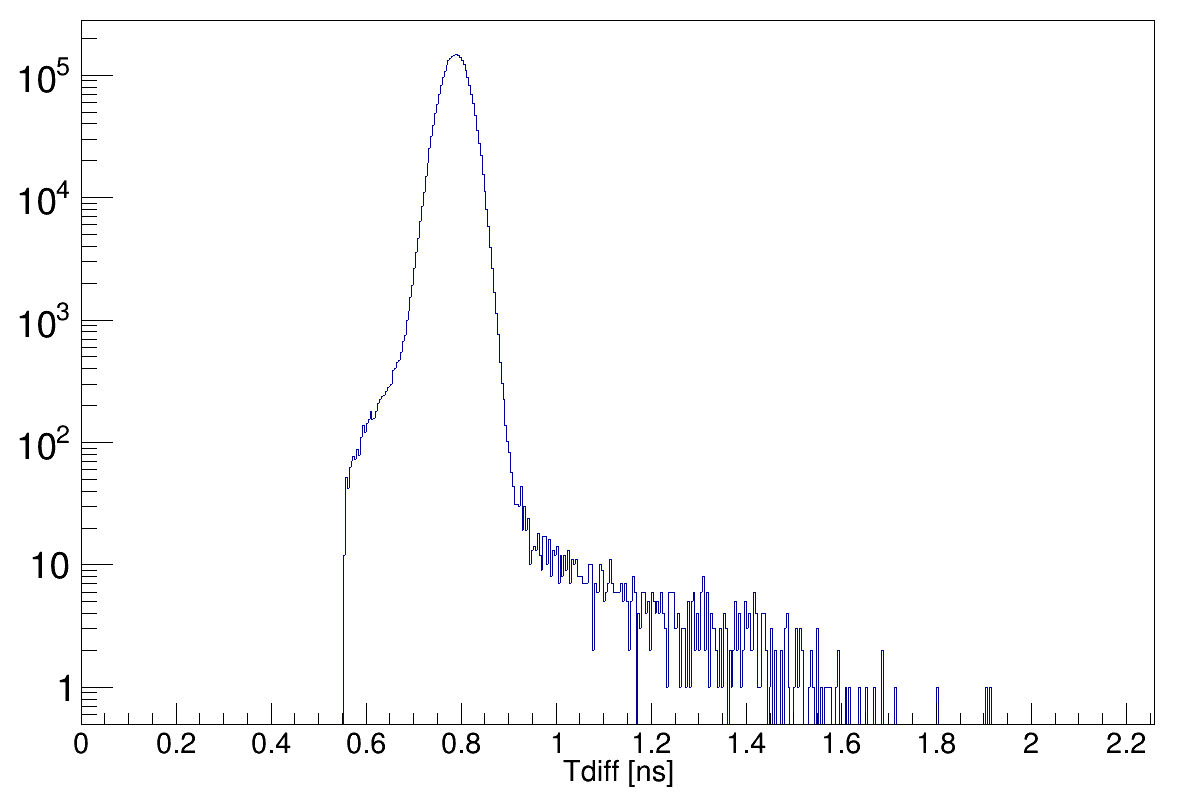
\includegraphics[width=\textwidth,height=8cm,keepaspectratio=true]{Figures/start_tdiff_exactly2good_hits.png}
\caption{$\Delta t_{right-left}$ between hits in the Start detector for events with exactly one hit on the left and right preamplifier and limiting the time differnce in the range 0.555 ns to 1.946ns.}
\label{fig:start_good_event_sel}
\end{figure}
\item \textbf{Projectile's focus on the active target region:}\newline
To assure that the incoming $^{12}$C ion hits the target it is necessary to select only events where the projectile is focussed to the active target region. Therefore strict cuts on the MWPC0 x and y positon are applied. This was achieved by fitting the x and y distribution of the MWPC0 (without any restrictions on it) by a gaussian function. The selection of good incoming events was then restricted to events with hits in MWPC0 within the $\pm 1\sigma$ region in the x and y position, see figure \ref{fig:mw0_xy_overview} and \ref{fig:mw0_cuts}.\newline
\begin{figure}
\centering
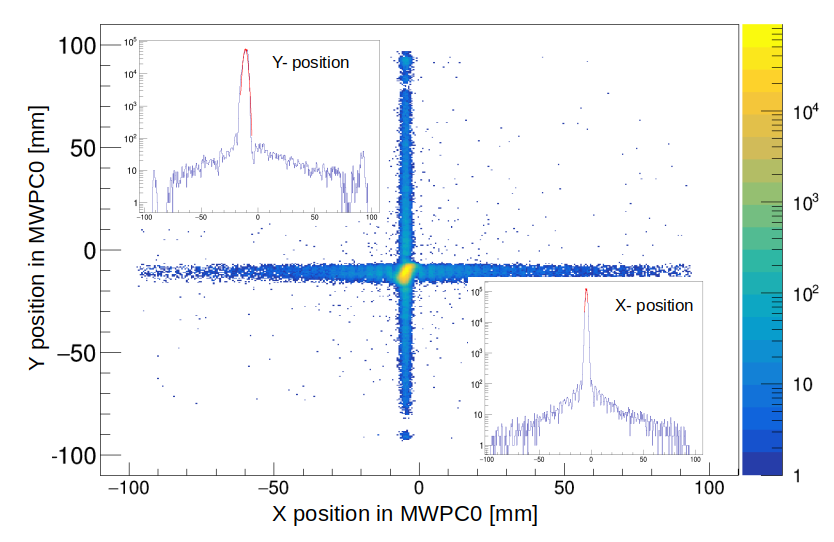
\includegraphics[width=\textwidth,height=8cm,keepaspectratio=true]{Figures/mw0_xy_summary.png}
\caption{x-y position of incoming ion on MWPC0.}
\label{fig:mw0_xy_overview}
\end{figure}
\begin{figure}
\centering
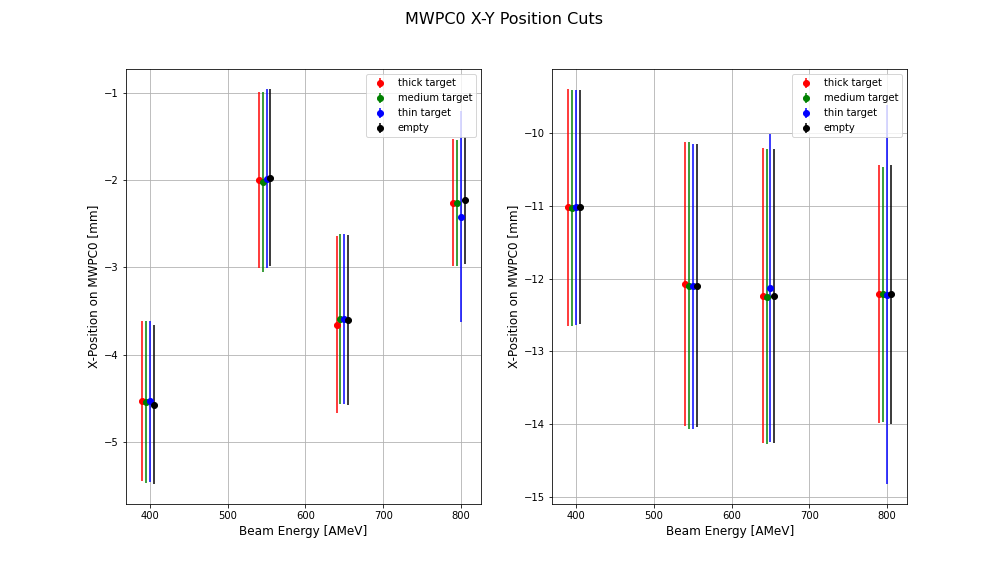
\includegraphics[width=\textwidth,height=8cm,keepaspectratio=true]{Figures/mwpc0_cutxy.png}
\caption{Overview of $\pm 1\sigma$ cuts in x and y in MWPC0 for empty/target runs.}
\label{fig:mw0_cuts}
\end{figure}
The MWPC0 x-position and the available projectile angle in the x-y plane from the R3BMusic is used to propagate the corresponding x-position on the target location to further check that the selected projectiles hit parallel to the z-position (= beam direction) the target and do only have a minimal incident angle,see figure \ref{fig:x_pos_target}. This can also be seen as a consistency check whether the applied (predefined) calibration parameters are properly set.
\begin{figure}[htpb]
    \centering
    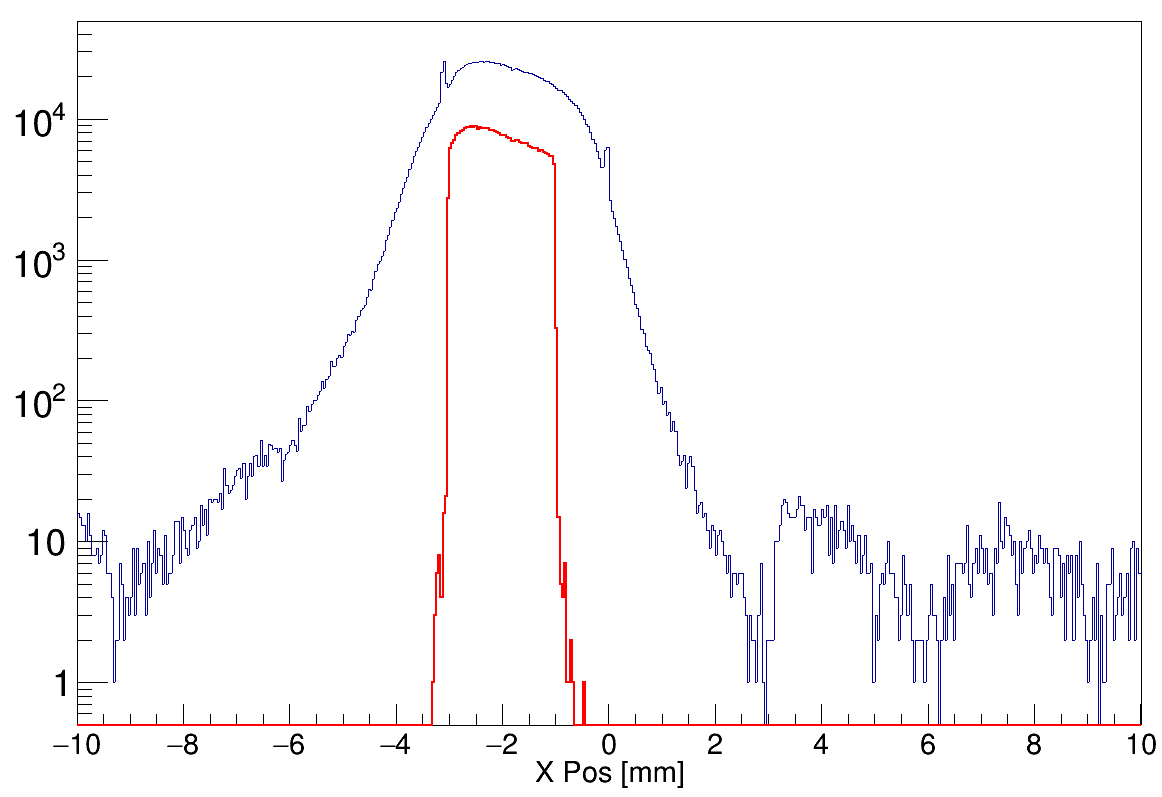
\includegraphics[width=\textwidth,height=8cm,keepaspectratio=true]{Figures/x_proj_beam_mw0_target.png}
    \caption{
   	Propagated x-position on target location from measured x-value on MWPC0 and x-y plane angle measurement from R3BMusic. The active target area is 3 x 3 cm. In red the selected events with $\pm 1\sigma$ cut in x and y position in MWPC0, in blue all events.
    }
    \label{fig:x_pos_target}
\end{figure}
\end{enumerate}
\subsection{Charge Changing Cross Section Measurement}
The charge changing cross section refers to a measure of the probability that the incoming projectile will undergo a reaction inside the target that changes its charge. To measure the charge changing cross section it can be referred to formula \ref{eq:corr_cross} where in this case $N_2$ is the number of survived carbon isotopes, i.e. projectiles which did not change their charge state. For this measurement only the data from the double ionisation chamber TWIN (see section \ref{sec:ionisation_chambers}) needs to be read out and analyzed.\newline
While for the event seletion before the target the cut conditions can be arbitrarly strict (it will only have an impact to the statistics and the derivated statistical error), cuts on the downstream detectors need to be avoided if at all possible. Too selective cuts on the identification of $N_2$ can distort the measurement.
\subsubsection{TWIN MUSIC Calibration}
For the analyis of data in TWIN MUSIC - different to the upstream detectors, where precalibrated data is used - the so called \textit{mapped} raw level data is processed. In the mapped level TWIN MUSIC provides following information:
\begin{itemize}
\itemsep0em 
\item \textbf{SectionID:} The detector is a double ionisation chamber and as such split up into four parts (in beam perspective): section 1 - right up; section 2 - right down; section 3 - left down; section 4 - left up. For the S44 experiment only section 1 was operated and accordingly centered on the beam spot.
\item \textbf{AnodeID:} TWIN MUSIC has 16 anodes for energy-loss readout and one refence anode (anodeID = 17).
\item \textbf{Time:} Each hit in each anode gets assigned to a time. Each time has individually no meaning. The drift time (in ns) of the electrons from the ionisation process of the gas by the inflying projectile (or the fragments of it) to the anode is calculated by substracting the individual anode time by the time of the reference anode. The reference anode gets its clean signal from a constant fraction discriminator of the START detector.
\item \textbf{Energy:} Each hit in each anode gets assigned to an energy - except the reference signal. To reconstruct the charge of the crossing through charged particle anodewise or detectorwise the parmetrization formula Z = [0] + [1]*$\sqrt(E)$ + [2]*E is used. 
\end{itemize}
The calibration of the TWIN energy for each anode is done run-wise. The event selection on the incoming ion is limited to the  \textit{"Min. Bias"} TPat condition (coincident signal in START detector peampliviers within 1.391 ns, on-spill). For the TWIN MUSIC only events where all anodes having exactly one hit (including the reference anode) are chosen. The most prominent peak (Z = 6) was fitted with gaussian function. The calibration was then done by determining the scaling factor for each anode  that shifts the mean of the gaussian fits to the same position, see figure \ref{fig:calibration}. For this analysis the peaks were shifted to $\Delta E = 6$. Since $\Delta E \propto Z^2$ holds, the scaled $\Delta E$ value, even though peaking at 6, is not equate the charge Z = 6.
\begin{figure}
     \centering
     \begin{subfigure}[t]{0.45\textwidth}
         \centering
         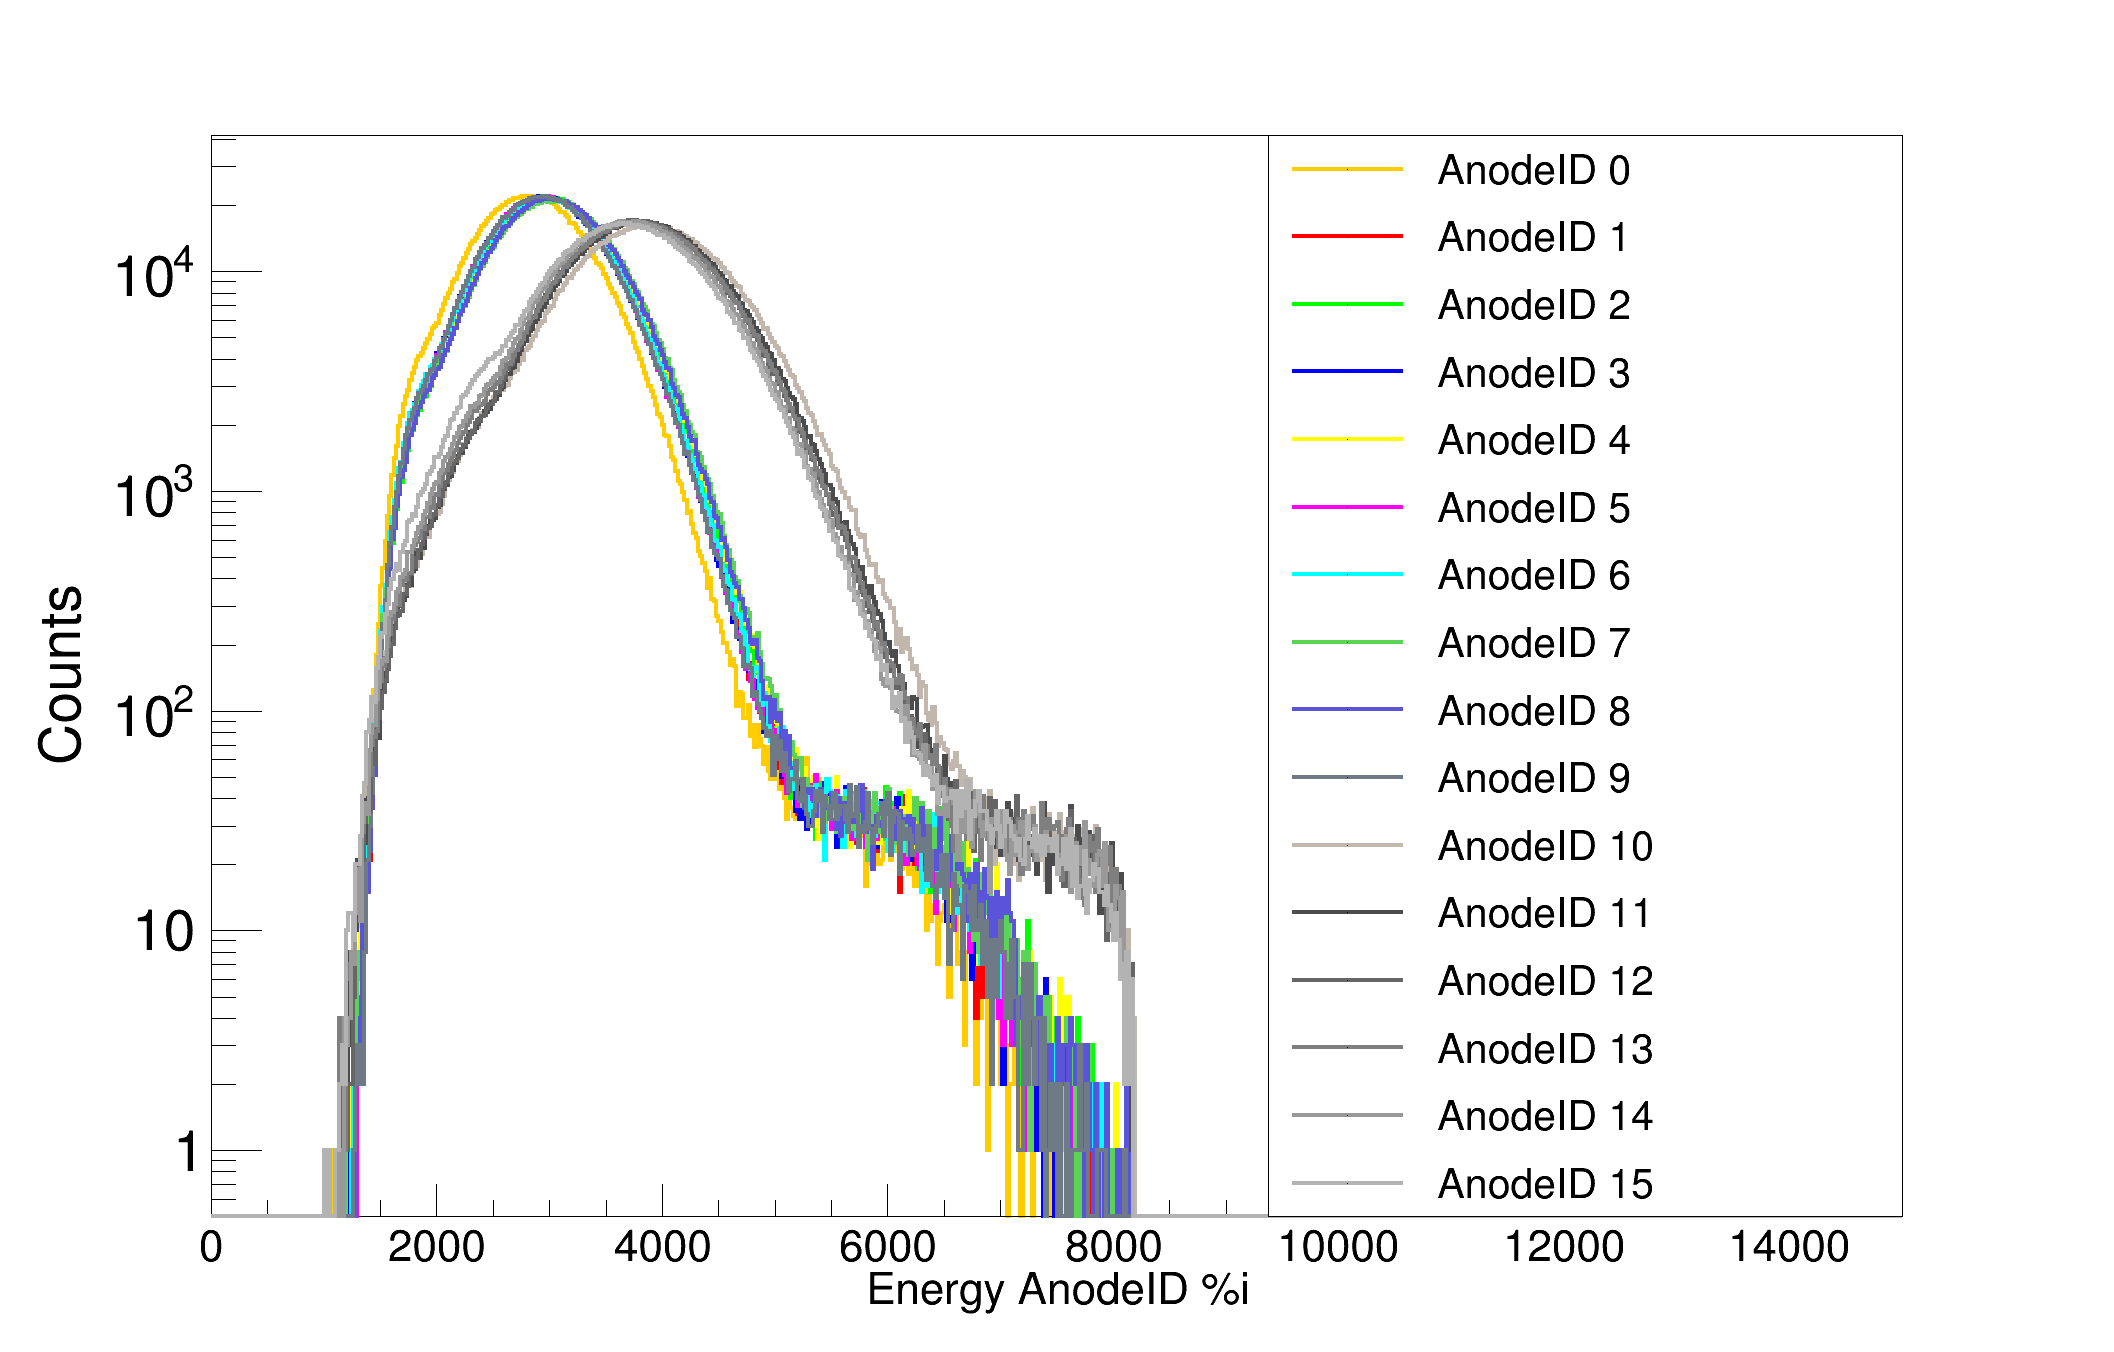
\includegraphics[width=\textwidth]{Figures/twim_mapped_550.png}
         \caption{Uncalibrated raw $\Delta E$ distributions for all 16 anodes for the 550 AMeV target run.The last six anodes have a slightly different electronics amplification chain.}
         \label{fig:raw_twim}
     \end{subfigure}
     \hfill
     \begin{subfigure}[t]{0.45\textwidth}
         \centering
         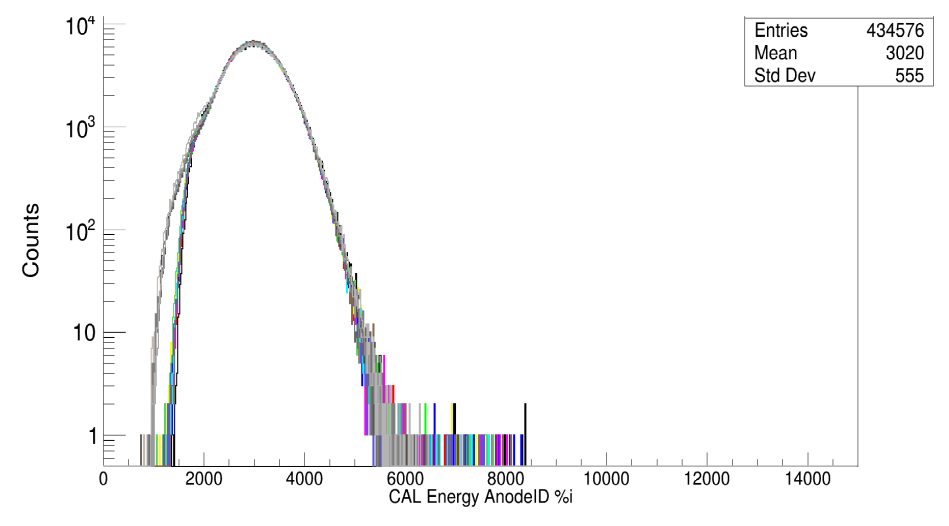
\includegraphics[width=\textwidth]{Figures/twim_mapped_550_no_calib.png}
         \caption{Gaussian fit applied to prominent peak and shifted to same position.}
         \label{fig:cal_twim_one}
     \end{subfigure}
     \hfill
        \caption{Fitting procedure in TWIN.TODO: nicer labeling!}
        \label{fig:calibration}
\end{figure}
\subsubsection{TWIN MUSIC Event Selection}
As previously stated cuts on the downstream detectors are avoided. However, events which have hits in one or several anodes in TWIN MUSIC but no signal in the reference anode are discarted as a whole neither contributing to $N_1$ (incoming selected ions) nor to $N_2$ (unreacted ions). If not reference time from START CFD signal is available it is not possible to measure the drift time in the individual anodes which makes it not possible to distinguish between signal and noise hits for multi-hit anode events in TWIN MUSIC. The number of events affected by this cut is in the region of few tens. This is negligible to the number of incoming ions $N_1$ and should not have any dependence whether the projectile reacted or not. 
\subsubsection{Carbon Identification}
The identification of carbon isotopes in TWIN is done by reconstructing fragments with charge Z = 6 from 2D plots where coincident mean energy losses $\Delta E$ for different anode combinations are plotted. Since the TWIN MUSIC is multi-hit capable various strategies were developed to deal with multi-hit events, i.e. when having anodes with multiple hits, decide which hit originates from the final state products from the reaction and which from background and noise.\newline
The default strategy is to use the time information of each hit for selection. It has to be remarked that for the S444 experiment the TWIN MUSIC was read out by two independent MDPP modules\cite{MDPP-16}. The signals from the first reference anode and the first eight upstream anodes were forwarded to module 1, the ones from the last eight downstream anodes and the second reference anode were forwarded to module 2. For the first eight upstream anodes the drift time is calculated by substracting the hit time in each anode by the reference time from the first reference anode and for the last eight downstream anodes accordingly the second reference andode was used:\newline
drift time formula
The time based selection algorithm for multi-hit anodes works as follows:\newline
\begin{enumerate}
\itemsep0em
\item Get the mean drift time for the eight upstream anodes($t_{mean\_up}$) and the eight downstream anodes($t_{mean\_down}$)\footnote{For the case all eight downstream anodes have multiple hits, set $t_{mean\_down} = t_{mean\_up}$ and vice versa}. Anodes with multiple hits do not contribute to this calculation.
\item If there are anodes with muliple hits compare the hit time with the accorging mean drift time ($t_{mean\_up}$ for any of the eight upstream anodes, $t_{mean\_down}$ for any of the eight downstream anodes). Calculate herefore the absolute difference between mean drift time and each hit time:
\begin{equation}
\Delta t = | \bar{t} - {t^i}_{drift}|;  \text{i = anodeID (1-16) with} \quad \bar{t} = 
\begin{cases}
t_{mean\_up} & \text{for i} \leq 8\\
t_{mean\_down} & \text{for i} \geq 9 \\
\end{cases}
\end{equation}
\item For each anodes with muliple hits select the hit with lowest drift time differnce to the mean drift time.
\end{enumerate}
\begin{figure}[htpb]
    \centering
    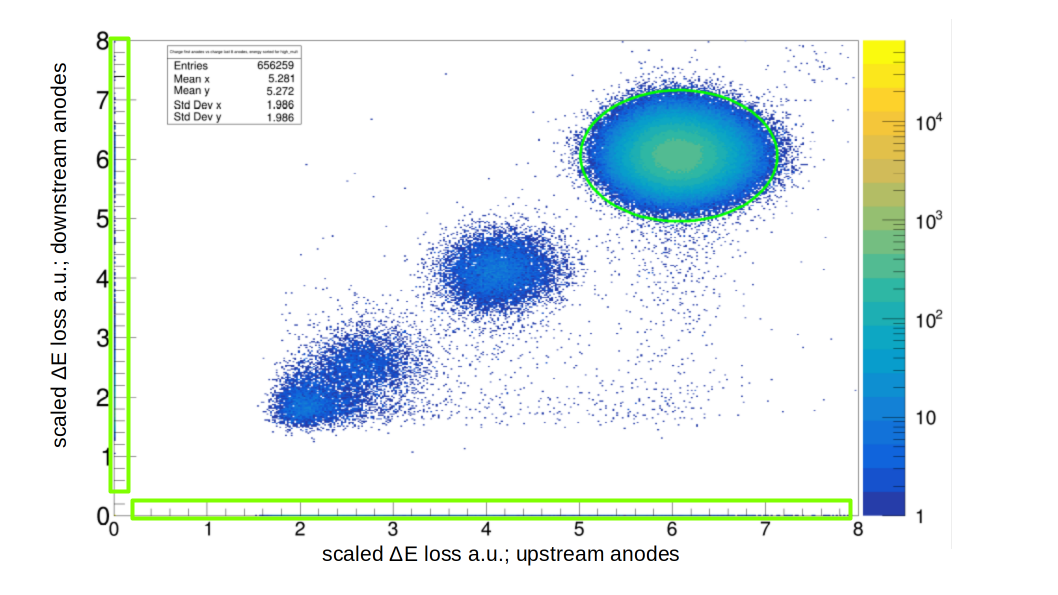
\includegraphics[width=\textwidth,height=8cm,keepaspectratio=true]{Figures/charge_cut_with_out_borders.png}
    \caption{
    Two dimensional gaussian fit with 3.5 $\sigma$ cut  on identified carbon isotopes in TWIN MUSIC. The horizontal and vertical side bars contain events where either the eight upstream anodes or downstream anodes have no hit entry.
    }
    \label{fig:twin_2d_gaus_cut}
\end{figure}

After having selected the appropriate hit for single and multi-hit anodes the mean value for the pre-calibrated $\Delta E$ loss, see figure \ref{fig:cal_twim_one}, for the eight upstream and accordingly for the eight downstream anodes is determined. Finally, to select the number of survived carbon isotopes the mean $\Delta E$ of the eight upstream anodes versus the mean $\Delta E$ of the eight downstream anodes is plotted. To retrieve the number of survived carbon isotopes following two-dimensional gaussian fit is applied on the 2D plot on the charge Z = 6 blob,see figure \ref{fig:twin_2d_gaus_cut}:
\begin{equation}
f(x) = A e^{-\frac{1}{2}((\frac{x - \bar{x}}{\sigma_{x}})^2 +(\frac{y - \bar{y}}{\sigma_{y}})^2)}
\label{eq:gauss_fit}
\end{equation},
where x is the mean rescaled energy loss of the first upstream andodes and y the according eight downstream anodes. The number of survived carbon isotopes is given by the integral of events within the 2D gaussian fit. Since the anodes were read out by two independent MDPP modules with slightly different thresholds also events along the histogram axes with no hit entry in either the upstream anodes or downstream anodes are analyzed. For those events a one dimensional gaussian cut is applied using the parameters from equation \ref{eq:gauss_fit}, see horizontal and vertical bars in figure \ref{fig:twin_2d_gaus_cut}.\newline
To get the charge changing cross section values equation \ref{eq:corr_cross} has to be applied where both the number of survived  carbon isotopes for target run and empty run are determined via the 2D gaussian fit as in figure \ref{fig:twin_2d_gaus_cut}. The number of target particles, $N_t$ in \ref{eq:corr_cross} is given by:
\begin{equation}
\begin{split}
&N_t = \rho \cdot N_A \cdot n \cdot d\\ 
&\rho = \text{density [$g/cm^3$]} = 1.851 g/cm^3,\text{taken from \cite{ponnath2023precise}}\\
&N_A = \text{Avogadro constant} =  6.02214076 \cdot 10^{23} mol^{-1}\\
&n = \text{amount of substance [mol/g]} = 1./12.011 \; mol/g\\
&d = \text{target thickness[cm]}
\end{split}
\end{equation}
Three carbon targets with different thicknesses are given:
\begin{enumerate}
\itemsep0em
\item thin target: d = 0.5451 cm
\item medium target: d = 1.0793 cm
\item thick target: d = 2.1928 cm 
\end{enumerate}
\begin{figure}[htpb]
    \centering
    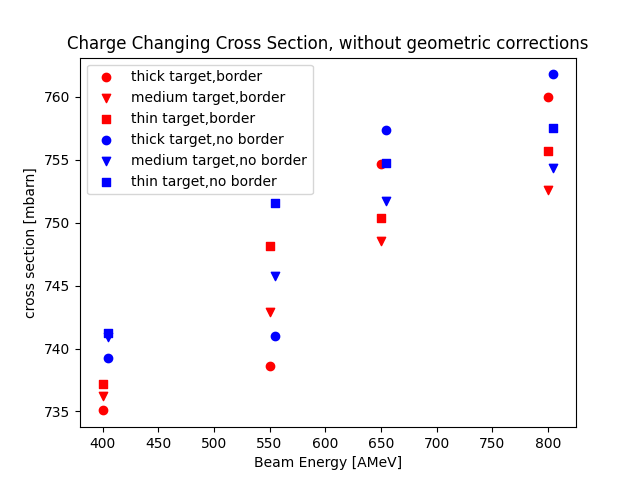
\includegraphics[width=\textwidth,height=8cm,keepaspectratio=true]{Figures/cccs_with_out_border_3_5_sigma.png}
    \caption{
    Charge changing cross section without geometry corrections. The red data points result from considering events with only hits in the upstream or downstream anodes, the blue data points don't take these events in consideration. 
     }
    \label{fig:cccs_with_out_border_3_5}
\end{figure}
The resulting charge changing cross sections are summarized in \ref{fig:cccs_with_out_border_3_5} once with consideration of the vertical/horizontal bars in figure \ref{fig:twin_2d_gaus_cut} and once without using a two dimensional gaussian fit with 3.5 $\sigma$ cut  on identified carbon isotopes. 
To get the optimal $\sigma$ cut on the two dimensional gaussian fit on the energy losses of the upstream anodes versus downstream anodes the charge changing cross section for all targets and all energies was systematically measured for $\sigma$-cuts in the range of 1 to 5 $\sigma$, see figure \ref{fig:cccs_vs_sigma_cut}. In the region $\thicksim$ 3.5$\sigma$ the variation of the cross section is minimal.
\begin{figure}[htpb]
    \centering
    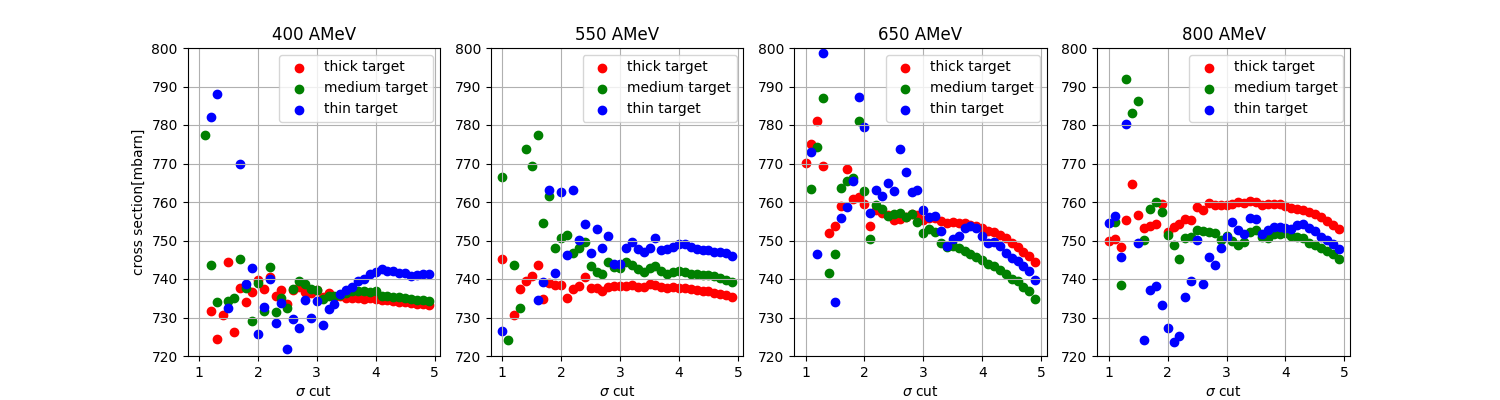
\includegraphics[width=\textwidth,height=8cm,keepaspectratio=true]{Figures/cccs_vs_sigma_cut.png}
    \caption{
    Measured charge changing cross sections according to the $\sigma$ cut applied on the figure \ref{fig:twin_2d_gaus_cut} (with borders) for the different target thicknesses and beam energies.
     }
    \label{fig:cccs_vs_sigma_cut}
\end{figure}
Another method to assert the number survived carbon ions is to apply a diagonal cut on the 2D $\Delta E$ histogram. To set the slope and offset of the diagonal cut line firstly the two dimensional gaussian fit is applied, same as for the previous method. Then the intersection point between the 3.5 $\sigma$ ellipse and the identity line ($\Delta E$ upstream anodes = $\Delta E$ downstream anodes) is found. Through this point, perpendicular to the identity line, the diagonal line is drawn. Everything above the diagonal line is considered as survived carbon ions. Moreover the borders are considered within the 3.5 $\sigma$ cut, see figure \ref{fig:diagonal_cut_twim}. 
\begin{figure}[htpb]
    \centering
    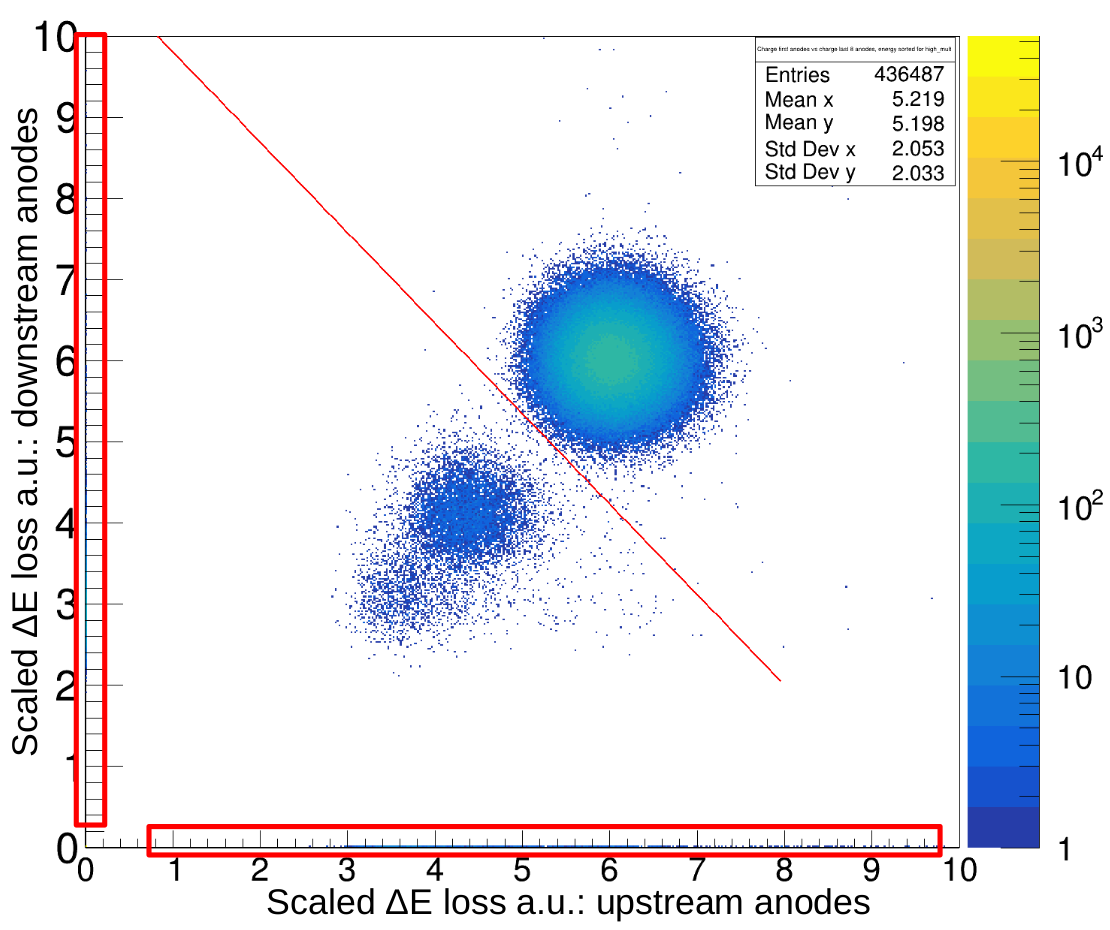
\includegraphics[width=\textwidth,height=8cm,keepaspectratio=true]{Figures/charge_loss_550_thick.png}
    \caption{
    Diagonal cut on identified carbon isotopes along the gaussian 3.5 $\sigma$ cut with borders. All hits above the diagonal line are counted as carbon isotopes. Histogram from thick target run, 550 AMeV beam energy.
     }
    \label{fig:diagonal_cut_twim}
\end{figure}
The effects of the different methods using to identify the carbon isotopes for the charge changing cross section is summarized in figure \ref{fig:cccs_gaus_vs_diag}. The differences in the measured cross sections are within the margin of error herefore both methods are comparable, as expected.
\begin{figure}[htpb]
    \centering
    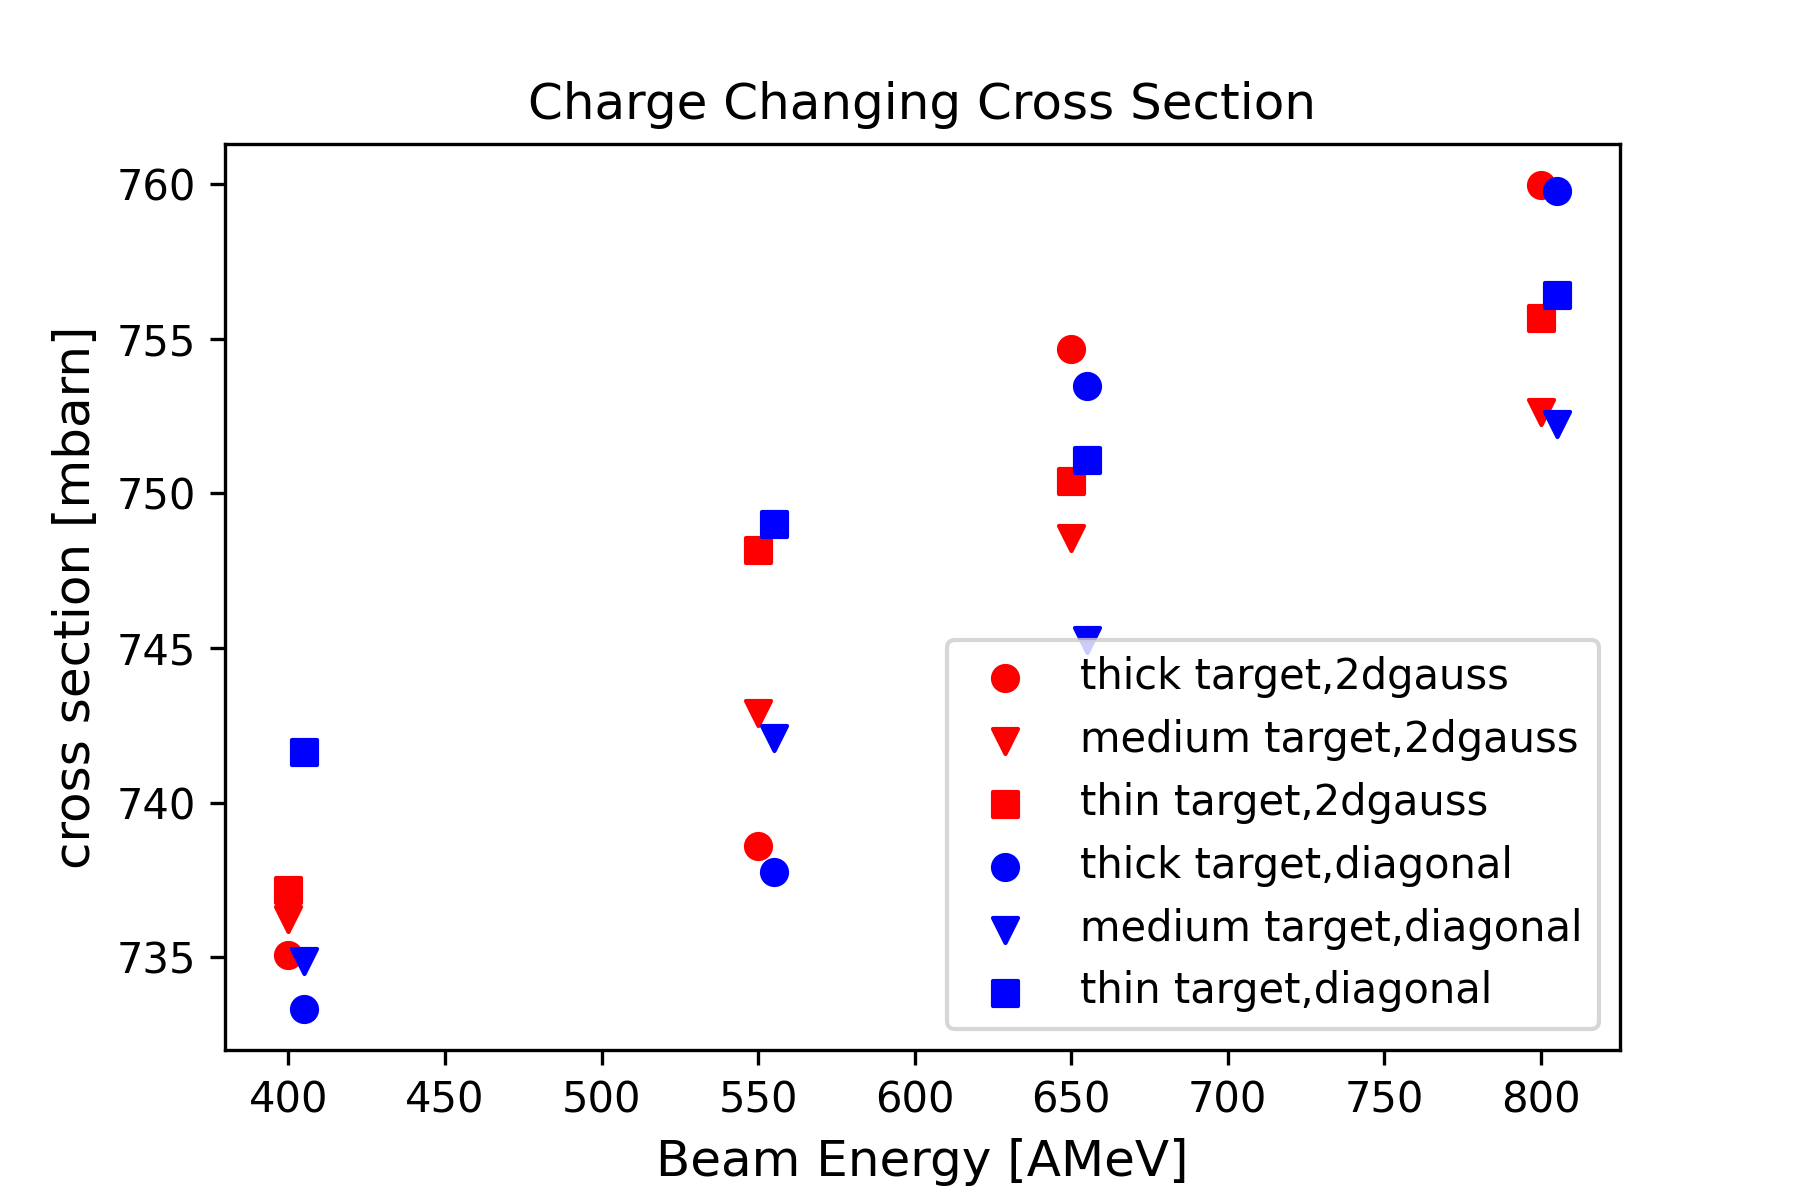
\includegraphics[width=\textwidth,height=8cm,keepaspectratio=true]{Figures/cccs_gauss_diag_comp_3_5_sigma.png}
    \caption{
    Comparison of charge changing cross section measured via 2D gaussian fit cut and diagonal cut. The differnces are within the margin of error.
     }
    \label{fig:cccs_gaus_vs_diag}
\end{figure}
To check wether single anodes or groups of anodes are malfunctioning the charge changing cross section measurement was repeated using only certain anodes for the charge identification:
\begin{enumerate}[label=\alph*)]
\itemsep0em
\item anodes 2-8 versus anodes 9-15 (omitting first and last anode)
\item anodes 1-4 versus anodes 5-8 (upstream anodes)
\item anodes 5-8 versus anodes 9-12 (central anodes)
\item anodes 9-12 versus anodes 13-16 (downstream anodes)
\end{enumerate}
The results from the measurement is summarized in figure \ref{fig:cccs_gaus_diff_sections}. The difference between the default gaussian fit method (with 3.5$\sigma$ cut and considering the borders) considering all 16 anodes and applying the same method but omitting the first and last anode is minimal over all four beam energies. When selecting only 8 out of 16 anodes instead the cross sections are systematically lower when going to high beam energies. TODO: give a good explanation about this divergence... 
\begin{figure}[htpb]
    \centering
    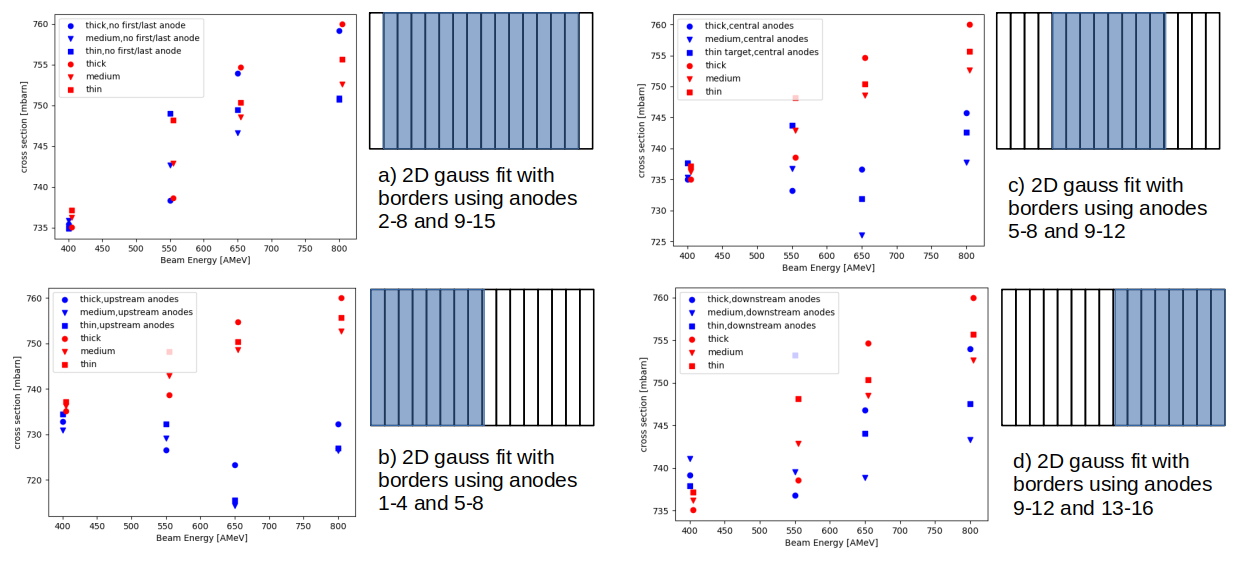
\includegraphics[width=\textwidth,height=8cm,keepaspectratio=true]{Figures/cccs_various_sections_2dgauss_border.png}
    \caption{
   	Measurement of charge changing cross sections using different anode sections to make the two dimensional gaussian fit on the identified carbon isotopes. Red: using all 16 anodes. Blue: the various combinations. 
     }
    \label{fig:cccs_gaus_diff_sections}
\end{figure}


%TODO:
%show method of taking different sections of TWIN DONE
%note that thickness calc from Lukas --TODO
%-> deltaE possonian distributed, according to central limit theorem, the sum too DONE
%-> therefore plot Esum of first 8 anodes vs Esum of last 8 anodes DONE
%-> two modules were used for readout DONE
%-> For selecting charge = 6 make gaussian fit on Esum up down DONE
%-> Compare charge = 6 cuts: DONE
%	-->show gaussian 2D cut, for all sigmas (with and whithout borders)
%	-->show gaussian diagonal cut for all sigmas (with and without borders)
%	-->show effect when discarting first/last, first two/last, first three/last and only using last 8 or last 6 anodes with fixed sigma cut
%	


\subsubsection{Results}



\subsection{Geometric Corrections}
\subsection{Isotope Correction - Total Interaction Cross Section}
\subsection{Fine Tuned Geometric Correction}
\subsection{Results}
\subsection{qfs analyis}
\subsection{reaction cross section Analysis}

